% !TeX document-id = {c15effce-b4cb-4262-806c-f65e49a6612b}
% !TeX TXS-program:compile = txs:///pdflatex/[--shell-escape]
\documentclass[mat1]{fmfdelo}
% \documentclass[fin1]{fmfdelo}
% \documentclass[isrm1]{fmfdelo}
% \documentclass[mat2]{fmfdelo}
% \documentclass[fin2]{fmfdelo}
% \documentclass[isrm2]{fmfdelo}

% naslednje ukaze ustrezno napolnite
\avtor{Laura Guzelj Blatnik}

\naslov{Nevronske mreže z vzvratnim razširjanjem napak v funkcijskem programskem jeziku}
\title{Feed-forward neural networks with backpropragtion in a functional programming language}

% navedite ime mentorja s polnim nazivom: doc.~dr.~Ime Priimek,
% izr.~prof.~dr.~Ime Priimek, prof.~dr.~Ime Priimek
% uporabite le tisti ukaz/ukaze, ki je/so za vas ustrezni
\mentor{prof.~dr.~Ljupčo Todorovski}
% \mentorica{}
 \somentor{asist.~dr.~Aljaž Osojnik}
% \somentorica{}
% \mentorja{}{}
% \mentorici{}{}

\letnica{2020} % leto diplome

%  V povzetku na kratko opišite vsebinske rezultate dela. Sem ne sodi razlaga organizacije dela --
%  v katerem poglavju/razdelku je kaj, pač pa le opis vsebine.
\povzetek{Diplomsko delo se poglobi v usmerjene nevronske mreže. Le te temeljijo na posnemanju možganskih funkcij, uporabljajo pa se za napovedovanje in klasifikacijo. Sestavljajo jih nevroni organizirani v sloje. Nevroni so med sabo povezani s sinapsami. S pomočjo algoritma za vzvratno razširjanje napake in učnih primerov mrežo naučimo odzivanja na neznane situacije. Algoritem temelji na spreminjanju uteži na sinapsah, učenje pa poteka dokler ni razlika med želeno in izračunano vrednostjo dovolj majhna. Poleg nevronskih mrež se delo osredotoči tudi na funkcijsko programiranje s poudarkom na programskem jeziku OCaml. Primer nevronske mreže z vzvratnim razširjanjem napak je tudi implementiran v programskem jeziku OCaml. Delovanje mreže je prikazano na konkretnem primeru, kjer je ovrednotena napaka mreže na izbrani podatkovni množici.}

%  Prevod slovenskega povzetka v angleščino.
\abstract{This paper focuses on feed-forward neural networks. Mimicking brain functions, neural networks are used for prediction and classification. Neural networks are composed of neurons organized in layers and connected by synapses. Utilizing the backpropagation algorithm and learning examples the network is able to learn how to respond to unknown situations. The idea behind backpropagation is to change weights on the synapses until the difference between computed and desired values is small enough. In addition, the work presents functional programming and the OCaml functional programming language. An implementation of a neural network with backpropagation in the OCaml programming language is presented at the end of the work. The work concludes with an application of the neural network to a real-world example, where the error of the network is evaluated on a specific data set.}

% navedite vsaj eno klasifikacijsko oznako --
% dostopne so na www.ams.org/mathscinet/msc/msc2010.html
\klasifikacija{68T05, 68N18}
\kljucnebesede{usmerjene nevronske mreže, vzvratno razširjanje napake, perceptron, umetna inteligenca, strojno učenje, funkcijski programski jezik OCaml} % navedite nekaj ključnih pojmov, ki nastopajo v delu
\keywords{feed-forward neural network, backpropagation, perceptron, artificial intelligence, machine learning, functional programming language OCaml}
 % angleški prevod ključnih besed

\zapisiMetaPodatke  % poskrbi za metapodatke in veljaven PDF/A-1b standard

% aktivirajte pakete, ki jih potrebujete
% \usepackage{tikz}

% za številske množice uporabite naslednje simbole
\newcommand{\R}{\mathbb R}
\newcommand{\N}{\mathbb N}
\newcommand{\Z}{\mathbb Z}
\newcommand{\C}{\mathbb C}
\newcommand{\Q}{\mathbb Q}

% matematične operatorje deklarirajte kot take, da jih bo Latex pravilno stavil
% \DeclareMathOperator{\conv}{conv}

% vstavite svoje definicije ...
%  \newcommand{}{}


\usepackage{minted}
\renewcommand\listingscaption{Algoritem}
\setminted{fontsize=\footnotesize}
\usepackage{neuralnetwork}
\usepackage{epstopdf}
\usepackage{graphicx}
\usepackage{geometry,color}
\usepackage{tikz}
\usetikzlibrary{matrix,chains,positioning,decorations.pathreplacing,arrows}
\usepackage{pgfplots}
\usepackage{pst-plot}
\psset{algebraic=true}

\usepackage{subcaption} 
\usepackage{nicefrac}

%\usepackage[ruled,vlined]{algorithm2e}


\begin{document}
%
\section{Uvod}
%
Človeški možgani so kompleksen organ predvsem zaradi neštetih funkcij, ki jih opravljajo. In zgolj vprašanje časa je bilo, kdaj bodo znanstveniki skoraj neskončne zmožnosti možganov prenesli v računalništvo. Ko so poskušali idejo uresničiti, so si predvsem želeli strukture, ki se bo -- podobno kot možgani -- sposobna učiti, odzivati na sprememe in prepoznavati neznane situacije. Tako je 1949 Donald Hebb v svojem delu The Organization of Behavior~\cite{hebb} prvič predstavil idejo o umetnih nevronskih mrežah, kjer se je zgledoval predvsem po možganih. 

Dvoslojni perceptorn, kot prva nevrosnka mreža zmožna učenja, se je rodil nekoliko kasneje, leta 1962 je ta pojem prvi omenil Frank Rosenblatt v Principles of Neurodynamics~\cite{rosenblatt}. Z razvojem strojne opreme se je zanimanje za nevronske mreže zopet povečalo v osemdesetih letih prejšnjega stoletja. Leta 1986 je več raziskovalcev neodvisno drug od drugega vpeljalo teorijo o večslojnih nevronskih mrežah in vzvratnem razširjanju napake. Kljub širokemu spektru uporabe, ki jih nudijo nevronske mreže, je interes zanje kasneje nekoliko upadel. V zadnjih letih pa so nevronske mreže zopet vroča tema, predvsem zaradi njihove zmožnosti prepoznavanja slik. Do danes so umetne nevronske mreže močno napredovale, namesto običajnih mrež se vedno bolj uporabljajo globoke nevronske mreže, ki so v nekaterih svojih zmožnostih primerljive z zmožnostmi možganov. Kljub vsemu pa so možgani sposobni masrcičesa, česar računalniki trenutno ne zmorejo.

Diplomska naloga se poglobi v usmerjene nevronske mreže in njihovo učenje z vzvratnim razširjanjem napake. Primer take mreže sem tudi implementirala v funkcijskem programskem jeziku OCaml. 
%
\section{Umetne nevronske mreže}
%
%
\subsection{Biološko ozadje}
Kot namiguje že samo ime, se umetne nevronske mreže v marsičem zgledujejo po človeških možganih. Osnovni gradniki možganov so nevroni, ki so med seboj povezani s sinapsami. Prav te goste povezave so ključne za delovanje živčevja. Skozi naše življenje se sinapse spreminjajo po jakosti in številu, ko se učimo se ustvarjajo nove povezave med nevroni, že obstoječe pa postajajo močnejše. Nevron se aktivira le,  ko po sinapsi do njega pride signal s točno določeno frekvenco, ta impulz nato nevron posreduje sosednjim nevronom. Človeške možgane sestavlja $10^{10}$ nevronov, vsak  ima približno $10^4$ sinaps. Umetne nevronske mreže načeloma sestavlja veliko manj gradnikov, posledično so pri izvajanju preprostih operacij veliko hitrejše od možganov. Kot bomo videli v nadaljevanju, je osnovna ideja umetnih nevronskih mrež zelo podobna živčevju v možganih. Lahko bi rekli, da so umetne nevronske mreže zgolj abstraktna poenosatvitev delovanja možganov. V nadaljnjem besedilu se izraz nevronske mreže nanaša na umetne nevronske mreže, besedo ''umetne'' bom zaradi kratkosti izpuščala.   
%
\subsection{Struktura nevronskih mrež}
Nevronske mreže so sestavljene iz nevronov, ki matematično gledano niso nič drugega kot funkcije. Nevroni so med seboj povezani s sinapsami, vsaka sinapsa ima svojo težo oziroma utež.
 Nevroni so organizirani v slojih. Nevroni v istem sloju med seboj niso povezani, vsak nevron je povezan z vsemi nevroni v naslednjem (oziroma prejšnjem sloju). Nevronska mreža vsebuje vhodni sloj nevronov, ti nevroni predstavljajo vrednosti vhodnih podatkov, in pa izhodni sloj nevronov, ki predstavlja izhodne vrednosti dobljene z nevronsko mrežo. V strojnem učenju se večinoma uporabljajo usmerjene nevrosnke mreže, kjer izračun vrednosti poteka od vhodnega sloja proti izhodnemu. Usmerjene nevronske mreže ne vsebujejo povratnih povezav, prav tako sinapse ne smejo tvoriti cikla.
 
 Nevronska mreža lahko vsebuje le vhodni in izhodni sloj -- takrat govorimo o dvoslojni nevronski mreži. Če se med tema slojema skriva še kakšen skriti sloj, potem mreža postane večslojna. Število nevronov v posameznem sloju kot tudi število skritih slojev nevronske mreže je odvisno od problema, ki ga nevronska mreža rešuje.
%
\begin{figure}
\centering
    \begin{neuralnetwork}[height=4]
        \newcommand{\x}[2]{$x_#2$}
        \newcommand{\y}[2]{$y_#2$}
        \newcommand{\hfirst}[2]{\small $h^{(1)}_#2$}
        \newcommand{\hsecond}[2]{\small $h^{(2)}_#2$}
        \inputlayer[count=3, bias=false, title=Vhodni\\sloj, text=\x]
        \hiddenlayer[count=4, bias=false, title=Skriti\\sloj 1, text=\hfirst] \linklayers
        \hiddenlayer[count=3, bias=false, title=Skriti\\sloj 2, text=\hsecond] \linklayers
        \outputlayer[count=2, title=Izhodni\\sloj, text=\y] \linklayers
    \end{neuralnetwork}
\label{mreza}
\caption{Perceptron z dvema skritima slojema nevronov}
\end{figure}
%
Pri mrežah, ki jih bom obravnavala v diplomski nalogi, so vse povezave usmerjene, čeprav je smiselno omeniti, da obstajajo tudi mreže z dvosmernimi povezavami. Usmerjeni nevronski mreži rečemo perceptron, glede na število slojev ločimo dvoslojni, tj.~perceptron z vhodnim in izhodnim slojem, in večslojni perceptron.  
%
\subsection{Delovanje perceptrona}
Vzemimo dvoslojni perceptron z $m$ nevroni v vhodnem sloju, njihova stanja in izhode\footnote{V vhodnem sloju so običajno izhodi nevronov enaki njihovim stanjem.} označimo z $X_1, X_2, \ldots, X_m$ in $n$ nevroni v izhodnem sloju, označimo jih $Y_1, Y_2, \ldots, Y_{n}$. Običajno sloj nevronov zapišemo v obliki vektorja:
%
\begin{equation*}
X = (X_1, X_2, \dotso, X_m)^\intercal  \quad \text{in} \quad  Y = (Y_1, Y_2, \dotso, Y_n)^\intercal \text{.}
\end{equation*}
%
Uteži med nevroni predstavimo z matriko:
%
\begin{equation*}
W = \begin{bmatrix}
W_{11} &W_{12}  & \cdots & W_{1m}  \\
W_{21}  &W_{22}  &\cdots & W_{2m}  \\
\cdots &  &\cdots &  \\
W_{n1} & W_{n2} & \cdots & W_{nm} 
\end{bmatrix}  
\end{equation*}
%
kjer element matrike $W_{ij}$ predstavlja utež med $j$-tim nevronom v vhodnem sloju in $i$-tim nevronom v izhodnem sloju.
%
\subsubsection{Funkcija kombinacije:}
Funkcijo kombinacije uporabljamo za izračun stanja $i$-tega nevrona na sledeč način:
%
\begin{equation*}
A_i= \sum_{j}W_{ij}X_j + C_i \text,
\end{equation*}
%
kjer je  $C_i$ konstanta aktivacije za $i$-ti nevron (njen pomen je pojasnjen v poglavju~\ref{bias}). 
Za cel sloj izhodnih nevronov pa lahko funkcijo kombinacije zapišemo z linearno preslikavo:
%
\begin{equation*}
A = WX \text,
\end{equation*}
%
kjer je $W$ matrika uteži, $X$ pa vhodni vektor. Če upoštevamo še konstante aktivacije, je potrebno matriko uteži $W$ in vektor $X$ malo preoblikovati. Vektorju na konec dodamo še eno komponento z vrednostjo $1$ in dobimo $X =  (X_1, X_2, \dotso, X_m, 1)^\intercal $ matriki uteži pa dodamo še stolpec s konstantami aktivacije za vsak nevron v izhodnem sloju, torej: 
%
\begin{equation*}
W = \begin{bmatrix}
W_{11} &W_{12}  & \cdots & W_{1m}  & C_1\\
W_{21}  &W_{22}  &\cdots & W_{2m}  & C_2\\
\cdots &\cdots  &\cdots &\cdots  &\cdots\\
W_{n1} & W_{n2} & \cdots & W_{nm} & C_n
\end{bmatrix}  
\end{equation*}
%
\subsubsection{Funkcija aktivacije:}
Cilj funkcije aktivacije je normalizirati vrednost, dobljeno s funkcijo kombinacije. Glede na namen uporabe nevronske meže lahko uporabimo različne funkcije aktivacije. Najpogosteje se uporabljaljata stopničasta pragovna funkcija ali pa sigmoidna funkcija. 

\emph{Stopničasta pragovna funkcija} nevron aktivira le, če je vrednost dobljena z funkcijo aktivacije nad oziroma pod določeno mejo. Uporaba te funkcije je dokaj omejena. Ker vhodnim podatkom pripiše le dve različni vrednosti, jo lahko uporabimo le pri klasifikaciji v dve kategoriji oziroma za reševanje linearnih problemov. Prav tako jo lahko uporabimo samo pri dvoslojnih perceptronih. Kot bomo videli v nadaljevanju, za večslojne perceptrone ni primerna, saj njen odvod ni gladek, kjer je definiran, pa je enak $0$, kar pa pomeni, da za učenje ne moremo uporabiti vzvratnega razširjanja napake. Primer stopničaste pragovne funkcije z izhodnima vrednostima $0$ in $1$ je:
%
\begin{equation*}
f(x)=
    \begin{cases}
      0, & \text{če } x  \leq 0 \\
      1, & \text{sicer.}
    \end{cases} 
\end{equation*}
%
\begin{figure}[!ht]
  \centering
    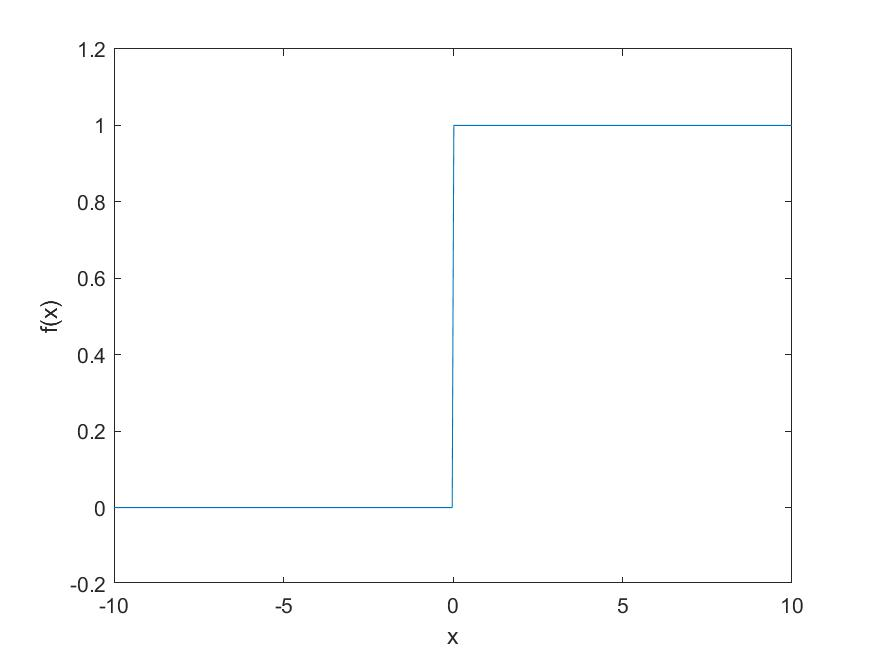
\includegraphics[width=0.5\textwidth]{step_fun.jpg}
  \label{fig:step}
 \caption{Stopničasta pragovna funkcija aktivacije}
\end{figure}

\emph{Sigmoidne funkcije} so nelinearne, zato se uporabljajo pri večslojnih perceptornih in reševanju nelinearnih problemov. So zvezne in neskončnokrat zvezno odvedljive, tako jih lahko uporabimo pri vzvratnem razširjanju napake. Odvisno na kateri interval želimo normalizirati izhodne vrednosti, lahko uporabimo različne sigmoidne funkcije. Primera sigmoidne funkcije sta: 
%
\begin{equation}
f(x) = \frac{1}{1+e^{-x}} \quad \text{in} \quad h(x) = \tanh(x) = \frac{e^x-e^{-x}}{e^x+e^{-x}} \text.
\end{equation}
%
Kot je razvidno z grafov (slika~\ref{fig:sigmoid}) je na intervalu $(-2,2)$ naklon obeh funkcij velik, zato na omenjenem intervalu mreža pri napovedovanju da jasne rezultate in učenje poteka hitro. Po drugi strani pa je zunaj tega intervala odvod majhen, tako je učenje mreže in posledično napovedovanje zelo počasno in nenatančno. 

Kot bomo videli v nadaljevanju, pri učenju mreže z vzvratnim razširjanjem napake potrebujemo tudi odvod funkcije aktivacije, saj le ta vpliva na posodabljanje uteži. Odvod uporabimo na že izračunanih stanjih nevronov, pri zgornijih dveh sigmoidnih funkcijah lahko preprosto izrazimo z $f(x)$ oziroma $h(x)$ na naslednji način:
%
\begin{equation}
f'(x) = \frac{e^{-x}}{(1+e^{-x})^2} = f(x)(1-f(x))
\end{equation}
%
\begin{equation}
h'(x) = \left(\frac{\sinh(x)}{\cosh(x)}\right)' = \frac{\cosh^2(x)- \sinh^2(x)}{\cosh^2(x)} = 1 - \tanh^2(x) = 1 - h(x)^2 
\end{equation}
%
\begin{figure}[!th]
\centering
\begin{subfigure}{.5\textwidth}
  \centering
  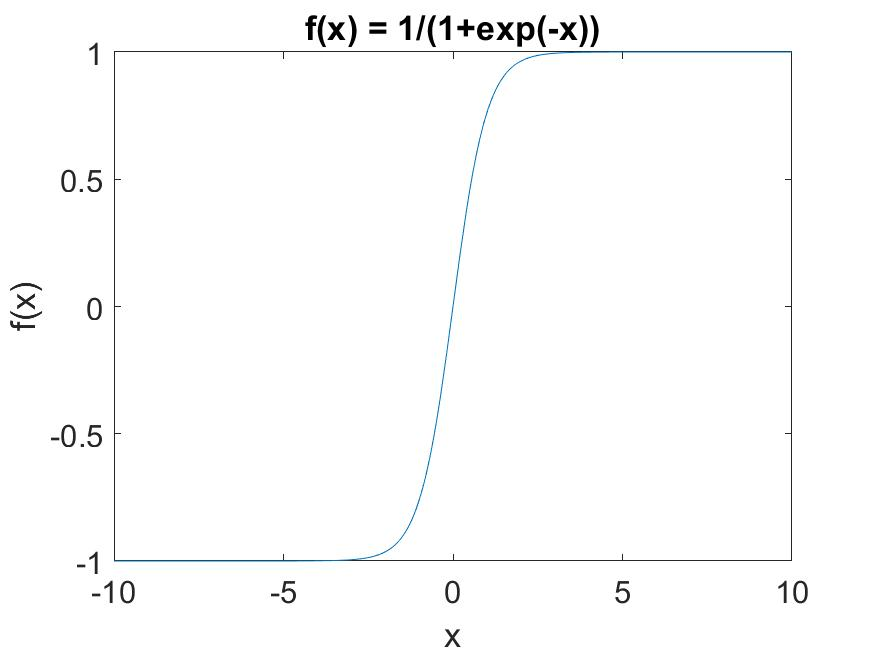
\includegraphics[width=.9\linewidth]{sig_exp.jpg}
\end{subfigure}%
\begin{subfigure}{.5\textwidth}
  \centering
  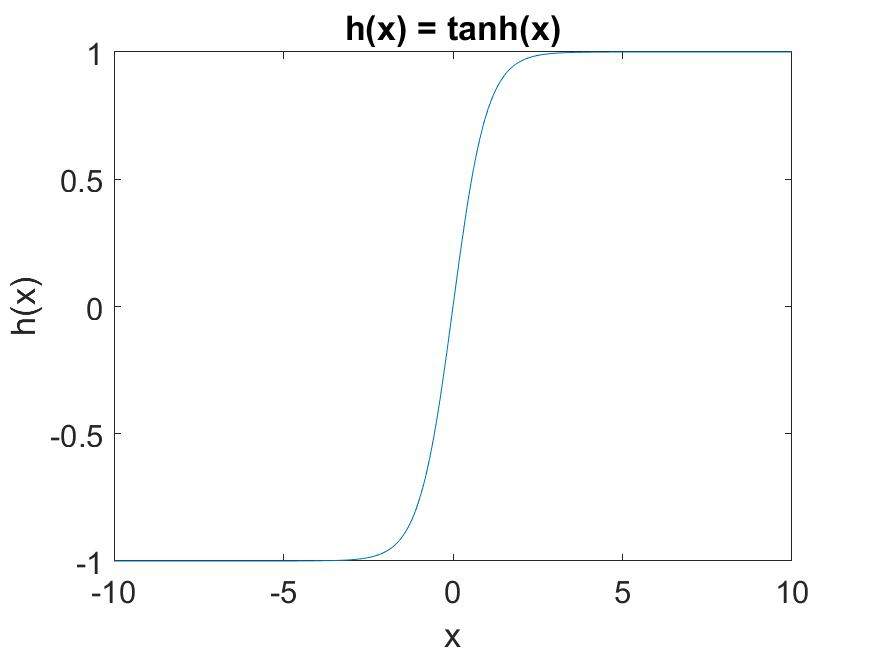
\includegraphics[width=.9\linewidth]{sig_tan.jpg}
\end{subfigure}
\caption{Sigmoidni funkciji aktivacije}
\label{fig:sigmoid}
\end{figure}
%

Katero funkcijo aktivacije bomo izbarli je odvisno od problema, ki ga želimo z mrežo obravnavati.
%
\subsubsection{Konstanta aktivacije} \label{bias}
Sloju nevronov pogosto dodamo še en nevron - konstanto aktivacije. To je nevron z izhodom $1$, ki posledično postane vhod za vse nevrone v naslednjem sloju. Naloga konstante aktivacije je, da funkcijo aktivacije primerno premakne levo oziroma desno po grafu. Brez dodatnega nevrona bi mreža pri vhodnem podatku $X=0$ vedno vračala vrednost $0$, posledično bi bila aproksimacija dane funkcije slaba in rezultati netočni. 

Pomen konstante aktivacije najlažje predstavimo s pomočjo linearne funkcije. Z enačbo oblike $y = kx$ lahko zapišemo le premice, ki prečkajo koordinatno izhodišče. Če pa fuknkciji dodamo še začetno vrednost, ki ustreza pomenu konstante aktivacije, potem lahko z enačbo $y= kx + n$ zapišemo poljubno premico. Z uporabo konstante aktivacije postane mreža bolj fleksibilna, problem bolje aproksimira in vrača bolj točne rezultate. 
%
\subsubsection{Funkcija nevrona}
Vrednost izhodnega sloja nevronov $Y$ dobimo tako, da na vhodnem nevronu najprej uporabimo funkcijo kombinacije in nato še funkcijo aktivacije -- obema funkcijama skupaj pravimo funkcija nevrona, tj., izračun izhodnih vrednosti nevrona. Za posamezen nevron velja:
%
\begin{equation*}
Y_i = f(\sum_{j}W_{ij}X_j + C_i)\text,
\end{equation*}
%
oziroma v vektorski obliki za cel sloj izhodnih nevronov:
%
\begin{equation*}
Y = f(WX) \text,
\end{equation*}
%
kjer velja, da funkcijo aktivacije uporabimo na vsaki komponenti vektorja $WX$. 
%
\begin{figure}
\centering
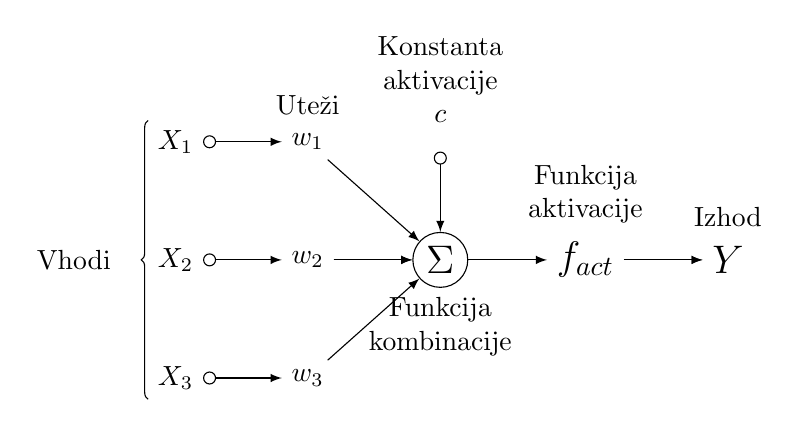
\begin{tikzpicture}[
    % define styles    
    init/.style={ 
         draw, 
         circle, 
         inner sep=2pt,
         font=\Huge,
         join = by -latex
    },
    squa/.style={ 
        font=\Large,
        join = by -latex
    }
]
% Top chain x1 to w1
\begin{scope}[start chain=1]
    \node[on chain=1] at (0,1.5cm)  (x1) {$X_1$};
    \node[on chain=1,label=above:Uteži,join=by o-latex] (w1) {$w_1$};
\end{scope}
% Middle chain x2 to output
\begin{scope}[start chain=2]
    \node[on chain=2] (x2) {$X_2$};
    \node[on chain=2,join=by o-latex] {$w_2$};
%\node[on chain=2,squa,label=above:{\parbox{6cm}{\centering Funkcija\\ kombinacije}}]{$\displaystyle\Sigma$};

    \node[on chain=2,init, squa,label=below:{\parbox{4cm}{\centering Funkcija\\ kombinacije}}] (sigma) {$\displaystyle\Sigma$};
    \node[on chain=2,squa,label=above:{\parbox{2cm}{\centering Funkcija\\ aktivacije}}]   {$f_{act}$};
    \node[on chain=2,squa,label=above:Izhod,join=by -latex] {$Y$};
\end{scope}
% Bottom chain x3 to w3
\begin{scope}[start chain=3]
    \node[on chain=3] at (0,-1.5cm) 
    (x3) {$X_3$};
    \node[on chain=3,join=by o-latex]
    (w3) {$w_3$};
\end{scope}
% Bias
\node[label=above:\parbox{2cm}{\centering Konstanta aktivacije \\ $c$}] at (sigma|-w1) (b) {};

% Arrows joining w1, w3 and b to sigma
\draw[-latex] (w1) -- (sigma);
\draw[-latex] (w3) -- (sigma);
\draw[o-latex] (b) -- (sigma);
% left hand side brace
\draw[decorate,decoration={brace,mirror}] (x1.north west) -- node[left=10pt] {Vhodi} (x3.south west);
\end{tikzpicture}
\caption{Funkcija nevrona (vhodi $X_1, X_2, X_3$ predstavljajo izhode nevronov iz prejšnjega sloja).}
\label{Funkcija nevrona}
\end{figure}
%
\subsection{Lastnosti nevronskih mrež}
Nevronske mreže odlikuje kar nekaj pozitivnih lastnosti. Najpomembnejše med njimi so sledeče:

\emph{Paralelizabilnost: }Posamičen nevron deluje relativno neodvisno od ostalih nevronov. To posledično omogoča paralelno računanje (znotraj sloja), v praksi pa to pomeni zelo hitre operacije. Zato lahko nevronske mreže uporabimo pri reševanju kompleksnih problemov.

\emph{Stabilnost: }Izgubljen ali nedelujoč nevron le malo pokvari natančnost delovanja nevronske mreže (več kot je takih nevronov, manj natančna je nevronska mreža). Nevronske mreže so tako stabilne v smislu uničenih nevronov in njihovih povezav. Poleg tega pa so stabilne tudi v smislu nepopolnih podatkov. To pomeni, da mrežo lahko naučimo pravilnega delovanja, tudi če v učnih priemrih del podatkov manjka. Velja pa, da bolj nepopolni kot so podatki, slabša je aproksimacija nevronske mreže.

\emph{Matematično ozadje: }Cilj nevronske mreže je aproksimirati poljubno funkcijo in kasneje na podlagi te aproksimacije napovedati vrednosti pri poljubnih vhodnih podatkih. Pri računanju se nevronske mreže močno opirajo na linearno algebro, linearnime preslikave, lastne vrednosti in vektorje ter negibne točke.\\

Glavna pomanjkljivost nevronskih mrež je težavno določanje topologije mreže. Medtem ko je število nevronov v vhodnem in izhodnem sloju določeno s problemom, je število nevronov v posameznem skritem sloju in število skritih slojev odvisno od posameznega primera. Idealno topologijo nevronske mreže je tako težko doseči, do nje lahko pridemo le s poskušanjem. Še ena slaba lastnost pa je nezmožnost razlaganja odločitev \emph{(ang.~black box model)}. Zaradi kompleksne strukture je vsak rezultat mreže produkt večih neodvisnih operacij nevronov, ki jih je težko razložiti.
%
%
\subsection{Uporaba nevronskih mrež}
Z razvojem strojne opreme v zadnjih letih so močno napredovale tudi nevronske mreže. Razvite so bile hitrejše implementacije algoritmov, posledično je zaradi njihove učinkovitosti uporaba nevronskih mrež danes zelo pogosta v industriji. Ko nevronsko mrežo naučimo pravilnega delovanja, se ta zna odzvati na nepoznane situacije. Tako lahko, zaradi njihove splošnosti in zmožnosti sprejetja velikega števila vhodnih podatkov, nevronske mreže uporabimo za reševanje najrazličnejših problemov. Nevronske mreže se dandanes uporabljajo na vseh mogočih področjih. Dva najpomembenjša namena uporabe sta napovedovanje in klasifikacija. Primeri uporabe v industriji so: 
\begin{itemize}
\item prepoznavanje in klasifikacija (delov) slik,
\item prepoznavanje ročno napisanih besedil,
\item prepoznavanje govora,
\item kontrola kvalitete v prozvodnji,
\item določanje diagnoz v zdravstvu,
\item napovedovanje različnih vrednosti glede na trenutne trende.
\end{itemize}
%
\section{Učenje nevronskih mrež}
Najprej je smiselno definirati, kaj pojem učenje sploh pomeni. Po~\cite[str.~37]{kononenko} za učenje potrebujemo sistem, ki strmi k izpolnitvi določene naloge oziroma cilja. Pred učenjem sistem ni sposoben zadostno opraviti naloge. S ponavljanjem določenih opravil poskušamo sistem pripraviti do tega, da bo deloval bolje, kjer je bolje lahko hitreje, ceneje, bolj pravilno\ldots\ Učenje lahko torej definiramo kot zaporedje ponovitev, kjer pri vsaki ponovitvi skušamo zmanjšati izbrano mero tako, da bi se zastavljenemu cilju čimbolj približali. 

Obstaja kar nekaj različnih pravil, kako umetno nevronsko mrežo naučiti pravilnega delovanja. V svoji diplomski nalogi sem se osredotočila na posplošeno pravilo delta oziroma vzvratno razširjanje napake, ki je najpogosteje uporabljan algoritem za učenje pri večslojnih perceptronih. 
%
\subsection{Nadzorovano učenje}
Vzvratno razširjanje napake je primer nadzorovanega učenja. Za tako učenje potrebujemo učne primere -- torej vhodne podatke in vrednosti, ki želimo, da jih mreža pri danih vhodnih podatkih vrača. Cilj učenja je najti funkcijo, ki bo najbolje aproksimirala relacijo med vhodnimi in izhodnimi podatki. Pri vzvratnem razširjanju napake do take funkcije pridemo tako, da spreminjamo vrednosti na utežeh, pri čemer poskušamo minimalizirati napako, tj., razliko med želenim in dejanskim izhodom mreže.

Potrebno je omeniti še, da poleg nadzorovanega učenja poznamo tudi nenazdrovano učenje. Tu izhodnih podatkov nimamo. Mreža vhodne podatke obdela po svojih kriterijih in poskuša najti strukturo, ki povezuje vhodne podatke med seboj. Nevroske mreže se za nenadzorovano učenje uporabljajo redkeje.
\subsection{Pravilo delta}
Pravilo delta je eno izmed pravil, ki ga lahko uporabimo pri učenju nevronske mreže, ponavadi se uporablja pri dvoslojnih perceptronih. Če je mreža večslojna, potem govorimo o vzvratnem razširjanju napake oziroma posplošenem pravilu delta. Za pravilom delta stoji povsem preprosta ideja. Najprej uteži med nevroni naključno nastavimo (pomembno je le, da niso vse uteži nastavljene na 0), nato na izbranem učnem primeru izračunamo, za koliko se je naša mreža zmotila glede na pričakovan izhod. Dobimo napako s pomočjo katere lahko vrednosti na utežeh popravimo tako, da omenjeno napako minimaliziramo. Postopek ponavljamo na ostalih učnih primerih, dokler se uteži ne ustalijo. Takrat se učenje konča.

Za začetek vzemimo preprost dvoslojni perceptron z enim izhodnim nevronom $Y$, število vhodnih nevronov je poljubno. Pravilo delta pri spreminjanju vrednosti uteži upošteva razliko med želenim in dobljenim izhodom mreže. Tako definiramo napako mreže $E(l)$ kot kvadrat razlike omenjenih vrednosti:
%
\begin{equation}
\begin{aligned}
E(l) &= (d(l)-Y(l))^2 \\
&= (d(l)-WX(l))^2
\label{eq:napaka}
\end{aligned}
\end{equation}
%
kjer je $d(l)$ želen izhod in $Y(l)= WX(l)$ z mrežo izračunana vrednost pri $l$-tem učnem primeru, vhodnem vektorju $X(l)$ in matriki uteži $W$.

Pravilo delta temelji na gradientnem iskanju -- vektor uteži popravljamo v negativni smeri odvoda napake po utežeh. Zaporedje takih popravkov nas namreč pripelje do lokalnega minimuma napake. Odvod napake po utežeh zapišemo sledeče:
%
\begin{equation*}
\frac{dE(l)}{dW}= -2(d(l)-WX(l))X(l)
\end{equation*}
%
Sedaj lahko zapišemo enačbo za pravilo delta in nove vrednosti uteži $W^{N}$:
%
\begin{equation}
\begin{aligned}
W^{N} &= W - \eta\frac{dE(l)}{dW} \\
&= W + \eta(d(l)-WX(l))X(l)
\label{utezi}
\end{aligned}
\end{equation}
%
V zgornji enačbi $\eta$ predstavlja hitrost učenja in vpliva na to, kako hitro bodo uteži konvergirale k optimalnim. 
%
\\

Zgoraj omenjeno \emph{gradientno iskanje} v resnici ni nič drugega kot iskanje lokalnega minimuma. Iskanje poteka tako, da začnemo na naključni točki na grafu (zato utežem na začetku pripišemo naključne vrednosti) in se nato v vsakem koraku premaknemo po krivulji v smeri negativnega odvoda, to je smer, kjer funkcija najhitreje pada. Dolžino vsakega premika določa stopnja učenja $\eta$, zato je pomembno kakšno vrednost zanjo izberemo. $\eta$ poleg hitrosti konvergence vpliva še na robustnost na lokalne
minumume - če je $\eta$ premajhen se lahko zgodi, da gradiento iskanje najde le najbližji lokalni minimum, ki pa morda ni optimalen. V nasprotnem primeru je prevelik $\eta$ preveč nestabilen, posledično lahko minimume povsem zgrešimo. Pomen izbire stopnje učenja je prikazan na sliki~\ref{fig:gradi}.
%
\begin{figure}[!ht]
	\centering
	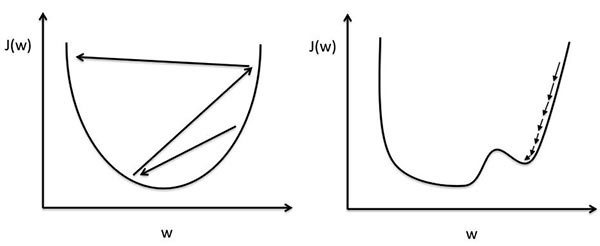
\includegraphics[width=0.5\textwidth]{gradient-descent.jpg}
	\caption{Vpliv prevelike oziroma premajhne stopnje učenja na iskanje lokalnega minimuma, vir~\cite{grad}}
		\label{fig:gradi}
\end{figure}

\subsection{Vzvratno razširjanje napake}
%IDEJA in opis
Vzvratno razširjanje napake je zgolj posplošitev pravila delta za večslojne perceptrone. Problem pri računanju se pojavi, ker uteži med skritimi sloji niso direktno odvisne od napake med izhodnim stanjem in želeno vrednostjo, zato moramo pravilo malo prilagoditi. Ko popravljamo uteži, to počnemo od izhodnega sloja nevronov proti vhodnemu (od tod tudi ime --  vzvratno razširjanje napake oz.\ \emph{backpropragation} v angleščini). 

\subsubsection{Notacija}
Definirajmo notacijo, ki jo bomo uporabili pri izpeljavi vzvratnega razširjavnja napake. 
\begin{itemize}
\item $X_{i}$ označuje vrednost oz.\ izhod $i$-tega nevron v vhodnem sloju.
\item $H_{ki}$ označuje vrednost oz.\ izhod $i$-tega nevrona v $k$-tem skritem sloju. 
\item $Y_i$ označuje vrednost oz.\ izhod $i$-tega nevrona v izhodnem sloju.
\item $W^{(k)}_{ij}$ označuje utež med $j$-tim nevronom v  $k-1$ plasti in $i$-tim nevronom v $k$-ti plasti.
\item $A_{ki}$ označuje stanje $i$-tega nevrona v $k$-ti skriti plasti po uporabljeni funkciji kombinacije: $A_{ki} = \sum^{N_{k-1}}_{j=1}W^{(k)}_{ij}H_{k-1,j}$, poseben primer je stanje $i$-tega nevrona v izhodni plasti, ki ga označimo z $A_i$.
\end{itemize}

\subsubsection{Izpeljava vzvratnega razširjanja napake}
Vzemimo splošen večsojen perceptron z $N_X$ nevroni v vhodnem sloju in $N_Y$ nevroni v izhodnem sloju. Nevronska mreža naj sestoji iz $m$ skritih slojev, $m>0$, vsak skriti sloj pa naj vsabuje $N_k$ nevronov, kjer velja $1\leq k \leq m$. 

Preden se lotimo popravljanja uteži, moramo za dani $l$-ti učni primer s pomočjo funkcije nevrona izračunati izhodne vrednosti. Za $i$-ti nevron v prvem skritem sloju lahko zapišemo:
%
\begin{equation*}
H_{1i}(l) = f\left( \sum^{N_X}_{j=1}{W^{(1)}_{ij}X_j(l)}\right)
\end{equation*}
%
in
%
\begin{equation*}
A_{1i}(l) =\sum^{N_X}_{j=1}{W^{(1)}_{ij}X_j(l)}\text.
\end{equation*}
%
Za poljubni $k$-ti sktiti sloj, kjer je $1\leq k \leq m$, tako zapišemo:
%
\begin{equation*}
H_{ki}(l) = f(A_{ki}(l))\text,
\end{equation*}
%
kjer je
%
\begin{equation*}
A_{ki}(l) = \sum^{N_{k-1}}_{j=1}W^{(k)}_{ij}H_{k-1,j}(l)\text.
\end{equation*}
%
V zgornji enačbi $H_{k-1,j}$ označuje že izračunane izhode nevronov v predhodnem sloju.
 
 V izhodnem sloju dobimo vrednosti, ki nas najbolj zanimajo. Velja:
%
\begin{equation*}
Y_{i}(l) = f(A_{i}(l)) \quad \text{in} \quad A_{i}(l) = \sum^{N_{m}}_{j=1}{W^{(m+1)}_{ij}H_{m,j}(l)}\text.
\end{equation*}
%
Tako smo dobili izhodne vrednosti, ki jih je izračunala mreža. Vrednosti primerjamo s tistimi, ki bi si jih želeli dobiti za dani $l$-ti učni primer. Za posamezen nevron ozančimo napako sledeče:
%
\begin{equation}
e_i(l) = d_i(l) - Y_i(l)\text,
\end{equation}
oziroma v vektorski obliki:
\begin{equation*}
e(l) = d(l) - Y(l)\text.
\end{equation*}
Podobno kot pri pravilu delta, definiramo napako celotne nevronske mreže za $l$-ti učni primer definiramo:
%
\begin{equation}
E(l) = \frac{1}{2}\sum^{N_Y}_{i=1}e_i^2(l)\text.
\label{napaka}
\end{equation}
%
Napako želimo minimalizirati in podobno kot prej s pomočjo gradientnega iskanja uteži popraviti v smeri njenega negativnega odvoda. Nove uteži izračunamo s pomočjo enake formule kot prej (enačba~\eqref{utezi}):
\begin{equation*}
W^{N} = W - \eta \frac{dE}{dW}, 
\end{equation*}
%
kjer $\eta$ označuje stopnjo učenja. 

Pri izračunu zgornjega odvoda si bomo pomagali s verižnim pravilom za odvajanje. Za izhodni sloj je napako enostavo izračunati. Problem se pojavi pri skritih slojih, saj uteži niso direktno odvisne od napake. Kot bomo videli v nadaljevanju, si bomo tudi v tem primeru pomgali z verižnim pravilom. 

Najprej razpišimo formulo~\eqref{napaka}, kjer upoštevamo formuli za $e_i$ in $Y_i$:
\begin{equation*}
\begin{aligned}
E(l) &= \frac{1}{2}\sum^{N_Y}_{i=1}e_i^2(l) \\
&=\frac{1}{2}\sum^{N_Y}_{i=1}{\left(d_i(l) - Y_i(l)\right)}^2 \\
&= \frac{1}{2}\sum^{N_Y}_{i=1}\left(d_i(l)-f\left(\sum^{N_m}_{j=1}W^{(m+1)}_{ij}H_{m,j}(l)\right)\right)^2
\end{aligned}
\end{equation*}
%
 Sedaj za izračun odvoda uporabimo verižno pravilo,  formulo razpišemo za posamezno utež:
%
\begin{equation}
\frac{\partial E(l)}{\partial W^{(m+1)}_{ij}} = \frac{\partial E(l)}{\partial e_i(l)}
\frac{\partial e_i(l)}{\partial Y_i(l)} 
\frac{\partial Y_i(l)}{\partial A_i(l)}
\frac{\partial A_i(l)}{\partial W^{(m+1)}_{ij}}
\end{equation}
%
Zgornje parcialne odvode pa lahko ob pomoči definicij posameznih izrazov zapišemo sledeče:
%
\begin{equation}
\frac{\partial E(l)}{\partial e_i(l)} = \frac{\partial}{\partial e_i(l)}\left(\frac{1}{2}\sum^{N_Y}_{i=1}e_i^2(l)\right)=e_i(l)
\end{equation}
%
\begin{equation}
\frac{\partial e_i(l)}{\partial Y_i(l)}= \frac{\partial (d_i(l) - Y_i(l))}{\partial Y_i(l)} = -1
\end{equation}
%
\begin{equation}
\frac{\partial Y_i(l)}{\partial A_i(l)} = \frac{\partial (f(A_i(l))) }{\partial A_i(l)} =f'(A_i(l))
\end{equation}
%
\begin{equation}
\frac{\partial A_i(l)}{\partial W^{(m+1)}_{ij}} =\frac{\partial}{\partial W^{(m+1)}_{ij}} \left(\sum^{N_m}_{j=1}W_{ij}^{(m+1)}H_{mj}(l)\right) = H_{mj}(l)
\end{equation}
%
Pri tem velja, da je $f'$ odvod funkcije aktivacije. 

Zaradi boljše preglednosti parcialni odvod zapišemo še malo drugače:
\begin{equation*}
\begin{aligned}
\frac{\partial E(l)}{\partial W^{(m+1)}_{ij}} = \frac{\partial E(l)}{\partial A_i(l)}\frac{\partial A_i(l)}{\partial W^{(m+1)}_{ij}} 
\end{aligned}
\end{equation*}
%
Če upoštevamo zgoraj izračunani odvod dobimo: 
%
\begin{equation*}
\frac{\partial E(l)}{\partial W^{(m+1)}_{ij}} = \frac{\partial E(l)}{\partial A_i(l)}H_{mj}(l) 
\end{equation*}
%
Označimo: 
%
\begin{equation}
\frac{\partial E(l)}{\partial A_i(l)} = \Delta^{(m+1)}_i(l)\text{,}
\label{eq:deltaY}
\end{equation}
%
kjer se $\Delta^{(m+1)}$ navezuje na stanja nevronov v izhodnem sloju.
%
Združimo vse zgornje rezultate in zapišemo:
%
\begin{equation}
\begin{aligned}
W^{N(m+1)}_{ij} &= W ^{(m+1)}_{ij}- \eta \frac{dE(l)}{dW_{ij}^{(m+1)}} \\
&= W ^{(m+1)}_{ij} -\eta  \Delta^{(m+1)}_i (l)H_{mj}(l)\\
&= W ^{(m+1)}_{ij} -\eta e_i(l) f'(A_i(l))H_{mj}(l)\\
\end{aligned}
\end{equation}
%
Tako smo izpeljali pravilo za spremembno uteži, ki povezujejo izhodni sloj s predhodnikom. 

Vzvratno razširjanje napake pride do izraza šele pri skritih slohjih. Ker ne moremo direktno izračunati napake $e_i$, si pri računanju pomagamo z že spremenjenimi utežmi v izhodnem sloju in pa $\Delta^{(m+1)}$, ki smo ga spotoma izračunali. Za uteži $W^{(m)}_{ij}$, ki povezujejo predzadnji in zadnji skriti sloj lahko ob upoštevanju verižnega pravila zapišemo:
%
\begin{equation*}
 \frac{\partial E(l)}{\partial W^{(m)}_{ij}} = \frac{\partial E(l)}{\partial A_{mi}(l)} \frac{\partial A_{mi}(l)}{\partial W^{(m)}_{ij}}
%= \Delta^{(m)}_i (l)H_{m-1,j}
\end{equation*}
%
Drugi člen odvoda izračunamo podobno kot prej
\begin{equation*}
\frac{\partial A_{mi}(l)}{\partial W^{(m)}_{ij}} = H_{m-1,j}(l)
\end{equation*}
%
in označimo
%
\begin{equation*}
\frac{\partial E(l)}{\partial A_{mi}(l)} = \Delta^{(m)}_i(l) \text.
\end{equation*}
%
Zopet uporabimo verižno pravilo za odvajanje in zapišemo:
%
\begin{equation*}
\Delta^{(m)}_i(l) = \frac{\partial E(l)}{\partial H_{mi}(l)}\frac{\partial H_{mi}(l)}{\partial A_{mi}(l)}
\end{equation*}
%
Drugi člen predstavlja odvod funkcije aktivacije:
%
\begin{equation*}
\frac{\partial H_{mi}(l)}{\partial A_{mi}(l)} =  f'(A_{mi}(l)) \text,
\end{equation*}
%
prvi člen pa ponovno razpišemo s pomočjo verižnega pravila sledeče:
%
\begin{equation*}
\begin{aligned}
\frac{\partial E(l)}{\partial H_{mi}(l)} &=  \sum^{N_Y}_{j=1} \frac{\partial E(l)}{\partial A_j(l)}\frac{\partial A_j(l)}{\partial H_{mi}(l)}  \\
& =   \sum^{N_Y}_{j=1} \frac{\partial E(l)}{\partial A_j(l)}\frac{\partial}{\partial H_{mi}(l)} \left(\sum^{N_m}_{p=1} W^{N (m+1)}_{jp}H_{mp}(l)\right)\\
&= \sum^{N_Y}_{j=1} \frac{\partial E(l)}{\partial A_j(l)} W^{N (m+1)}_{ji}
\end{aligned}
\end{equation*}
%
Pri tem velja, da so elementi matrike uteži $W^{N(m+1)}$ vrednosti, ki smo jih že popravili v prejšnjem koraku. Uporabimo enačbo~\eqref{eq:deltaY} in izrazimo vrednost $\Delta^{(m)}_i(l)$ sledeče:
%
\begin{equation*}
\begin{aligned}
\Delta^{(m)}_i(l) &= f'(A_{mi}(l))  \sum^{N_Y}_{j=1} \frac{\partial E(l)}{\partial A_j(l)} W^{N (m+1)}_{ji} \\
&= f'(A_{mi}(l))  \sum^{N_Y}_{j=1} \Delta ^{(m+1)}_j(l)W^{N (m+1)}_{ji}
\end{aligned}
\end{equation*}
%
Vse združimo in vstavimo v enačbo za izračun spremenjenih uteži $W^{N(m)}$ ter dobimo:
%
\begin{equation}
\begin{aligned}
W^{N(m)}_{ij} &= W^{(m)}_{ij} - \eta\frac{dE(l)}{dW_{ij}^{(m)}} \\
&= W ^{(m)}_{ij} -\eta  \Delta^{(m)}_i (l)H_{m-1,j}(l)\\
&= W ^{(m)}_{ij} -\eta f'(A_{mi}(l))  \left(\sum^{N_Y}_{p=1} \Delta ^{(m+1)}_p(l)W^{N (m+1)}_{pi}\right)H_{m-1,j}(l)\\
\end{aligned}
\end{equation}
%
Za uteži $W^{(k)}$, ki povezujejo poljuben $k-1$ in $k$-ti skriti sloj, kjer je $1 < k < m$, podobno zapišemo:
%
\begin{equation*}
\frac{\partial A_{ki}(l)}{\partial W^{(k)}_{ij}} = H_{k-1,j}(l)
\end{equation*}
%
in 
%
\begin{equation*}
\Delta^{(k)}_i(l) =  f'(A_{ki}(l))  \sum^{N_{k+1}}_{j=1} \Delta ^{(k+1)}_j(l)W^{N (k+1)}_{ji}
\end{equation*}
%
Spremenjene uteži nato izračunamo:
%
\begin{equation}
\begin{aligned}
W^{N(k)}_{ij}&= W ^{(k)}_{ij} -\eta  \Delta^{(k)}_i (l)H_{k-1,j}(l)\\
&= W ^{(k)}_{ij} -\eta f'(A_{ki}(l))  \left(\sum^{N_{k+1}}_{p=1} \Delta ^{(k+1)}_p(l)W^{N (k+1)}_{pi}\right)H_{k-1,j}(l)\\
\end{aligned}
\end{equation}
%
Ostane nam le še matrika uteži $W^{(1)}$, ki povezuje vhodni sloj s prvim skritim slojem. Tu velja:
%
\begin{equation*}
\frac{\partial A_{1i}(l)}{\partial W^{(1)}_{ij}} = X_j(l)
\end{equation*}
%
in 
%
\begin{equation*}
\Delta^{(1)}_i(l) =  f'(A_{1i}(l))  \sum^{N_{2}}_{j=1} \Delta ^{(2)}_j(l)W^{N (2)}_{ji}
\end{equation*}
%
Uteži pa popravimo po sledeči formuli:
%
\begin{equation}
\begin{aligned}
W^{N(1)}_{ij}&= W ^{(1)}_{ij} -\eta  \Delta^{(1)}_i (l)X_j(l)\\
&= W ^{(1)}_{ij} -\eta f'(A_{1i}(l))  \left(\sum^{N_{2}}_{p=1} \Delta ^{(2)}_p(l)W^{N (2)}_{pi}\right)X_j(l)\\
\end{aligned}
\end{equation}
%
%
Tako smo izpeljali pravilo za računanje spremembe uteži pri vzvratnem razširjanju napake.
%
\subsection{Lastnosti vzvratnega razširjanja napake}
Kljub temu, da je vzvratno razširjanje napake zelo priljubljeno pravilo pri učenju nevronskih mrež, ima tudi nekaj pomanjkljivosti. 

Gradientno iskanje temelji na iskanju lokalnega minimuma, posledično uteži ne konvergirajo vedno k globalno najboljši izbiri. Lahko se zgodi, da bo matrika uteži konvergirala k lokalnemu optimumu, taka mreža ne bo dajala zadovoljivih rezultatov. Kam bodo uteži konvergirale je odvisno predvsem od njihove začetne izbire. Če med učenjem pride do omenjenega problema moramo izbrati novo naključno matriko uteži in učenje ponoviti v upanju, da bodo uteži tokrat konvergirale k optimalnim.

Naslednji problem, ki se pojavi kot posledica gradientnega iskanja je določanje parametra $\eta$. Stopnja učenja vpliva na to kako hitro in kam bodo uteži konvergirale. Žal pa ni pravila, ki bi določalo kakšno vrednost je za $\eta$ najbolje izbrati. Do take vrednosti lahko pridemo le s poskušanjem.

Slabost vzvratnega razširjanja napake je tudi to, da je za učenje nevronske mreže potrebno zelo veliko število učnih primerov. Ponavadi se to število giblje med nekaj $10000$ in $100000$. Posledično je učenje lahko zelo zamudno.

Potrebno je omeniti še časovno zahtevnost. Zaradi svoje kompleksne zgradbe so nevronske mreže časovno potratne in njihovo učenje praviloma ni hitro. Z večjo mrežo le to zahtevnost še povečamo. Kljub temu pa lahko z različnimi implementacijami do neke mere vplivamo na hitrost učenja mreže.

Včasih se lahko zgodi, da napaka mreže med učenjem začne naraščati. Pomembno je, da učenje takrat prekinemo, saj lahko sicer pride do preprileganja \emph{(ang. overfitting)}. Preprileganje pomeni, da mreža zelo dobro deluje na učnih primerih (napaka je tu majhna), aproksimacija za poljuben primer izven množice učnih primerov pa ni natančna. Zato je pomembno, da med učenjem ves čas spremljamo vrednost napake na primerih iz posebne množice testnih primerov, ki jih ne uporabljamo za učenje.
%
\subsection{Pristranskost in varianca}
Po končanem učenju lahko izračunamo pristranskost \emph{(ang. bias)} in varianco nevronske mreže. Ti vrednosti povesta, kako uspešni smo bili pri aproksimaciji funkcije oziroma učenju nevronske mreže. Ker gre za aproksimacijo, bo pristranskost vedno prisotna, želimo pa si, da bi bila le ta čim manjša. Omenjeni količini izračunamo s pomočjo testnih primerov.

S $t$ označimo točno vrednost, ki bi jo želeli dobiti, s $\hat{t}$ pa vrednost, ki jo mreža vrne. Z $\operatorname{E}[\hat{t}]$ označimo pričakovano vrednost napovedi, to je povprečna vrednost napovedi modelov naučenih iz različnih učnih množic. Pristranskost mreže pri $t$-tem učnem primeru označimo z $N(t)$ in izračunamo sledeče:
%
\begin{equation}
N(t) = \operatorname{E}[\hat{t}] - t \text.
\end{equation}
%
Problem se pojavi, če točne vrednosti $t$ ne poznamo. Včasih lahko iz ostalih podatkov sklepamo, kakšna bi ta vrednost morala biti ali pa jo poskusimo oceniti na drugačen način. Pristranskost meri, kako dobro mreža deluje na učnih primerih. Majhna pristranskost pomeni, da je bilo učenje uspešno in da bo vsaj napoved na učnih primerih in primerih, ki so učnim podobni, dobra. Če je pristranskost prevelika jo zmanjšamo tako, da izberemo večjo nevronsko mrežo.

Nadalje definiramo še varianco
%
\begin{equation}
Var(\hat{t}) = \operatorname{E}[\operatorname{E}[\hat{t}] -\hat{t}]^2\text.
\end{equation}
%
Kot je razvidno iz zgornje enačbe, $Var(\hat{t})$ ni odvisna od točnih vrednosti $t$. Varianca meri  občutljivost napovedi na spremembe učne množice. Stremimo k temu, da bi bila varianca čim manjša. Če je le ta prevelika, jo zmanjšamo tako, da povečamo število učnih primerov, vendar to ni vedno mogoče. Če je varianca še vedno velika, lahko poskusimo tudi z drugačno topologijo mreže.

Spomnimo se, kako se glasi napaka, ki jo pri posplošenem pravilu delta želimo minimalizirati. Če enačbo napake (enačba~\eqref{napaka}) prepišemo v smislu novo označnih količin, dobimo:
%
\begin{equation}
\begin{aligned}
\operatorname{E}[(\hat{t}-t)^2] &= \operatorname{E}[(\hat{t} -\operatorname{E}[\hat{t}] + \operatorname{E}[\hat{t}] - t)^2]  \\
\end{aligned}
\end{equation}
Upoštevamo še $\operatorname{E}[t] = t$ in $\operatorname{E}[\operatorname{E}[\hat{t}]\hat{t}] = \operatorname{E}[\hat{t}]^2$ in zapipšemo:
\begin{equation}
\begin{aligned}
\operatorname{E}[(\hat{t}-t)^2] &= (\operatorname{E}[\hat{t}] - t)^2 +\operatorname{E}[\operatorname{E}[\hat{t}] -\hat{t}]^2\\
&= N(t)^2 + Var(\hat{t})
\end{aligned}
\end{equation}
%
Iz zgornje enačbe vidimo, da sta pristranskost in varianca mreže tesno povezani med seboj in da z učenjem mreže poskušamo minimalizirati njuno vsoto. Pri minimumu napake mreže pa se vseeno lahko dobimo različne vrednosti omenjenih parametrov. Poglejmo si, kako te vrazlične vrednosti vplivajo na delovanje mreže.
%
\begin{figure}[!ht]
  \centering
    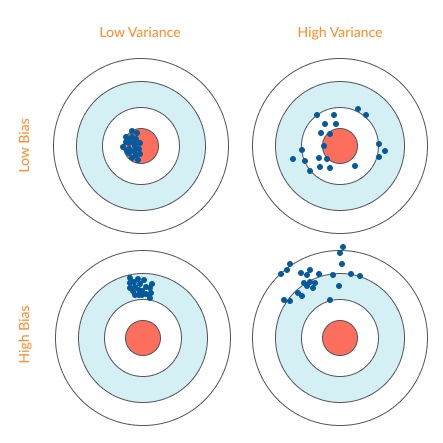
\includegraphics[width=0.5\textwidth]{bias.jpg}
  \label{fig:bis}
 \caption{Pristranskost \emph{(ang.~bias)} in varianca \emph{(ang.~variance)}, vir~\cite{bias}}
\end{figure}
%

Če bomo izbrali kompleksno topologijo nevronske mreže (torej veliko število skritih plasti in nevronov - globoko mrežo) bo pristranskost majhna, a zaradi občutljivosti velikega števila uteži na male spremembe učne množice je varianca lahko zelo visoka. Zato v takem primeru obstaja nevarnost preprileganja. To pomeni, da bo mreža zelo dobro delovala na učnih podatkih, ne bo pa sposobna znanja posplošiti na poljubne vhodne podatke.
Po drugi strani pri izboru enostavne topologije (torej topologije z malim številom skritih plasti in nevronov) opazujemo visoko pristranskost, a hkrati nizko varianco -- v takih situacijah obstaja resna možnost neprileganja (ali podprileganja, \emph{ang.~underfitting}). Taka mreža ne bo sposobna dobro aproksimirati niti učnih podatkov, na dobro napoved splošnih podatkov lahko pozabimo.

Če pride do preprileganja, moramo učenje ponoviti, le da tokrat izberemo drugačne vrednosti začetnih uteži. Postopek ponavljamo, dokler z delovanjem mreže nismo zadovoljni. Neprileganje lahko odpravimo tako, da spremenimo topologijo mreže. Lahko dodamo oziroma odstranimo nevrone, sloje ali pa dodamo kakšen parameter v vhodni sloj nevronov. Prav tako lahko dodamo nekaj učnih primerov oziroma izboljšamo njihovo kakovost. Načeloma velja, da na več učnih primerih kot bomo mrežo učili, bolje bo mreža delovala.
%
\subsection{Normalizacija podatkov}
Različne vhodne vrednosti imajo lahko različne enote in se razlikujejo za kar nekaj velikostnih redov. Taki podatki pri učenju ne bodo dali dobrih rezultatov. Da optimiziramo delovanje mreže, je podatke pred učenjem potrebno normalizirati oziroma pretvoriti v enak velikostni red. Želimo si, da bi bili podatki majhni, tako bo učenje boljše. Obstaja več pravil za normalizacijo podatkov, najbolj pogosti sta min-max normalizacija in z-score normalizacija, ki jo včasih imenujemo tudi standarizacija. Kako bomo podatke normalizirali je odvisno od primera, ki ga obravnavamo.
%
\subsubsection{Min-max normalizacija}
Podatke normaliziramo po sledeči enačbi:
%
\begin{equation}
X_{norm} = \frac{X -X_{min}}{X_{max}-X_{min}}
\end{equation}
%
Tako podatke skrčimo na interval $[0,1]$. 
%
\subsubsection{Z-score normalizacija}
Cilj je podatke preoblikovati tako, da bomo dobili strandardno normalno porazdelitev z povprečjem $0$ in standardnim odkolonom $1$. To dosežemo, če podatke preoblikujemo po sledeči enačbi:
%
\begin{equation}
X_{norm} = \frac{X - \mu}{\sigma} \text,
\end{equation}
%
pri čemer velja, da je $\mu$  povprečna vrednost in $\sigma$ standardni odklon podatkov.
%
\section{Funkcijski programski jezik OCaml}
Poleg funkcijskih poznamo še objektne in proceduralne programske jezike. Vsi načini programiranja imajo svoje prednosti in slabosti. Funkcijsko programiranje je zelo priljubljeno za pisanje generičnih algoritmov in algoritmov, ki temeljijo na rekurziji. 

Način programiranja in programski jezik izberemo na podlagi več dejavnikov -- včasih izberemo tak jezik, da bo program deloval kar se da hitro, drugič izberemo jezik v katerem bo zastavljeni problem najlažje rešljiv.
Sama sem se za OCaml odločila, ker so implementacije nevronskih mrež v funkcijskih programskih jezikih zelo redke in mi je to predstavljalo izziv. 
%
\subsection{Lastnosti funkcijskih programskih jezikov}
V funkcijskem programiranju so osnovni objekti funkcije. To pomeni, da lahko funkcije sprejmejo ozrioma vračajo druge funkcije, poleg tega lahko funkcije shranimo v podatkovne strukture. Funkcijam, ki kot argument sprejmejo druge funkcije pravimo \emph{funkcije višjega reda}. Ena izmed osnovnih funkcij višjega reda je na primer funkcija \texttt{map}. Le ta sprejme podatkovno strukturo, naprimer seznam ali tabelo, in na vsakem njenem elementu uporabi funkcijo, ki smo jo podali kot argument.
%
\begin{listing}[!h]
\begin{minted}[fontsize=\normalsize]{ocaml}
val activation_layer : ('a -> 'b) -> 'a array -> 'b array = <fun>
let activation_layer funct layer =
	Array.map funct layer
\end{minted} 
\caption{Primer uporabe funkcije map, ki funkcijo aktivacije uporabi na sloju nevronov, ki ga podamo s tabelo}
\label{algoritem}
\end{listing}
%%

\emph{Čiste funkcije} so pomemben koncept v funkcijskem programiranju. Funkcija je \emph{čista} \emph{(ang. pure function)}, če med izvajanjem ne sproži nobenih stranskih učinkov kot so npr.\ izpisovanje na zaslon, branje z tipkovnice, spreminjanje vrednosti spremenljivk\ldots\ Poleg tega čiste funkcije pri enakih argumentih vedno vračajo enak rezultat, posledično lahko tako funkcijo vedno zamenjamo z njeno definicijo.  Čiste funkcije v praksi pomenijo manj napak med programiranjem, če se le te že pojavijo, jih je lahko najti in odpraviti. V funkcijskem programiranju je večina funkcij čistih, saj funkcije načeloma vrednosti ne spreminjajo, ampak jih vračajo. 
\subsection{Lastnosti OCamla}
OCaml je splošen programski jezik, kljub temu da ima veliko lastnosti funkcijskih jezikov. Poleg le teh, ima OCaml tudi lastnosti objektnega programiranja. 
Posledično OCaml odlikuje kar nekaj pozitivnih lastnosti. Izvajanje kode je hitro in učinkovito, jezik ima velik poudarek tudi na varnosti, preden izvajanjem programa prevajalnik kodo preveri, zato do sintaktičnih napak le redko prihaja.

Funkcije v OCamlu so večinoma čiste, ne drži pa to vedno. S pomočjo referenc lahko namreč spreminjamo vrednosti spremenljivk. Zaradi narave nevronskih mrež sem to lastnost pri implementaciji izkoristila kar nekajkrat.

Dobra lastnost OCamla je tudi, da optimizira repno rekurzijo. Klic funkcije je repen, če se izvede zadnji. Pri rekurziji gre omeniti še OCamlovo sposobnost efektivnega ujemanja vzorcev. 

OCaml ima dobro podprt sistem tipov. Tipi v OCamlu so statični, a se tudi tej lastnosti v določenih situacijah da izogniti z referencami. Jezik omogoča pisanje polimorfnih funkcij, tako da le te delujejo na poljubnem tipu vhodnih podatkov, kar je pri programiranju dostikrat zaželjeno. 
%
%
%-tipi
%- nespremenljivi tipi, to ni vedno ok -> rešitev so reference
%
%\subsection{Tipi in moduli}
\section{Implementacija nevronske mreže}
Del diplomske naloge je bila tudi implementacija usmerjene nevronske mreže v programskem jeziku OCaml. Cilj je bil implementirati generičen večslojni perceptron z vzvratnim razširjanjem napake. Nadalje sem nevronsko mrežo tudi testirala na dani podatkovni množici in jo analizirala. Celotna implementacija se nahaja na koncu naloge, v prilogi~\ref{priloga}, prav tako pa je dostopna tudi na povezavi \url{https://github.com/lauraguzeljblatnik/nevronske-mreze}.
%
\subsection{Primer nevronske mreže}
Glavna funkcija, ki poskrbi, da se mreža nauči delovanja je funkcija  \texttt{train\_network}. Funkcija vrne tabelo matrik naučenih uteži med sloji, sprejme pa naslednje vhodne podatke:
\begin{itemize}
	\item \texttt{input\_array}: tabela vhodnih vektorjev,
	\item \texttt{output\_array}: tabela pripadajočih želenih izhodnih vektorjev,
	\item \texttt{network\_topology}: tabela, ki opisuje topologijo mreže s št. nevronov po slojih,
	\item \texttt{rate}: stopnja učenja,
	\item \texttt{bound}: meja, ki določa maksimalno vrednost začeno nastavljenih naključnih uteži,
	\item \texttt{act\_fun}: funkcija aktivacije,
	\item \texttt{act\_der}: odvod funkcije aktivacije.
\end{itemize}
%
Signatura funkcije se glasi:
%
\begin{listing}[!h]
	\begin{minted}[fontsize=\normalsize]{ocaml}
val train_network :
	float array array -> float array array -> int array -> 
	float -> float -> (float -> float) -> (float -> float) -> 
	float array array array =
<fun>
	\end{minted} 
	\caption{Signatura funkcije \texttt{train\_network}}
	\label{signatura}
\end{listing}

Nadalje s pomočjo funkcije \texttt{predict} in naučenih uteži napovemo vrednosti za poljubne vhodne podatke. Le ta sprejme tabelo \texttt{input}, ki predstavlja vektor vhodnih podatkov, matriko \texttt{network}, ki predstavlja nevrone v nrevronski mreži, matriko matrik \texttt{weights}, ki predstavlja uteži med posameznimi sloji in funkcijo aktivacije \texttt{act\_fun}, ki jo želomo uporabiti. Funkcija vrne tabelo, ki predstavlja vekor napovedanih vrednosti. Signatura je tako:
%
\begin{listing}[!h]
	\begin{minted}[fontsize=\normalsize]{ocaml}
val predict :
	float array ->
	float array array ->
	float array array array -> (float -> float) -> 
	float array = 
<fun>
	\end{minted} 
	\caption{Signatura funkcije \texttt{predict}}
	\label{signatura2}
\end{listing}
%
\subsection{Vrednotenje na podatkovni množici}
Delovanje nevronske mreže sem preverila na podatkovni množici, ki sem jih pridobila s spletnega naslova \url{https://archive.ics.uci.edu/ml/datasets/bike+sharing+dataset}.

 Vse fun\-kci\-je, ki sem jih uporabila pri analizi delovanja nevronske mreže so vključene v nalogo in se nahajajo v prilogi~\ref{priloga}.
%
\subsubsection{Podatkovna množica o izposoji koles}
Podatkovna množica vsebuje informacije o številu izposojenih koles za posamezen dan med letoma $2011$ in $2012$ v sistemu Capital Bikeshare v mestu Washington D.~C. Število izposojenih koles je odvisno od naslednjih vhodnih podatkov: 
\begin{itemize}
	\item letni čas: $1$ - zima, $2$ - pomlad, $3$ - poletje, $4$ - jesen
	\item leto: $0$ - leto $2011$, $1$ - leto $2012$
	\item mesec: $1$ do $12$
	\item praznik: $1$, če je bil dan praznik, $0$ sicer
	\item dan v tednu: $0$ do $6$, $0$ predstavlja nedeljo
	\item delovni dan: $1$, če je dan delovni, $0$ če je praznik ali vikend
	\item vreme: $1$ - jasno, posamezni oblaki, delno oblačno, $2$ - meglice, posamezni oblaki, oblačno,  $3$ - rahel sneg, rahel dež z razpršenimi oblaki, rahel dež v nevihtami, $4$ - nalivi, toča, nevihte, sneg, megla
	\item temperatura: vrednosti so podane v stopinjah celzija in normalizirane sledeče: $t=\nicefrac{(t-t_{min})}{(t_{max}-t_{min})}$, kjer je $t_{min}=-8$, $t_{max}=+39$
	\item občutek mraza: vrednosti so podane v stopinjah celzija in normalizirane sledeče: $t=\nicefrac{(t-t_{min})}{(t_{max}-t_{min})}$, kjer je $t_{min}=-16$, $t_{max}=+50$
	\item vlažnost: normalizirana vrednost vlažnosti, vrednosti so deljene s $100$, kar je maksimalna vrednost
	\item veter: normalizirana hitrost vetra, vrednosti so deljene s $67$, kar je maksimalna vrednost
\end{itemize}

Uporabniki koles so razdeljeni na občasne in registrirane uporabnike, tako podatkovni nabor vsebuje informacije o številu obeh skupin in njuni vsoti. Izhodni podatki so torej:
\begin{itemize}
	\item število občasnih uporabnikov,
	\item število registriranih uporanikov,
	\item število vseh uporabnikov (občasnih in registriranih).
\end{itemize}

Nabor podatkov vsebuje informacije o izposoji koles za $731$ dni, od tega sem prvih $600$ primerov uporabila za učenje, na $131$ primerih pa sem preverjala delovanje nevronske mreže.
%
\subsubsection{Analiza delovanja nevronske mreže}
Delovanje mreže sem preverjala s pomočjo povprečne absolutne nakake. Namesto kvadrata napake sem izbrala absolutno napako. Absolutna napaka se meri na isti skali kot vrednosti same, posledično se jo lažje interpretira. Za učenje mreže pa absolutna napaka ni primerna, ker nima gladkega odvoda in se je ne da lepo optimizirati, zato tam uporabimo kvadrat napake. Povprečno absolutno napako sem izračunala tako, da sem za vsak testni primer izračunala napako med želeno vrednostjo in vrednostjo napovedano s pomočjo nevronske mreže. Formula za izračun napake močno spominja na enačbo \eqref{eq:napaka}, za $l$-ti učni primer se enačba glasi:
%
\begin{equation*}
E(l) = |d(l)-Y(l)|\text.
\end{equation*}
%
 Nato sem vzela povprečje teh napak za vse testne primere in tako dobila povprečno absolutno napako sledeče:
 %
 \begin{equation}
 E_{povp}(l) = \frac{1}{n}\sum_{i=1}^{n}|d(l)-Y(l)|\text,
 \end{equation}
 %
 kjer $n$ predstavlja število testnih primerov.
 
  Da bi bili izračuni kar se da robustni glede na naključno izbrano začetno stanje, sem učenje mreže ponovila na petdesetih različnih začetnih utežeh in na koncu izračunala povprečje vseh napak. Napako sem računala posebej za vsakega izmed izhodnih parametrov.

S pomočjo funkcije \texttt{learned\-\_vs\-\_unlearned} pokažemo uspešnost učenja nevronske mreže. Funkcija za $n$ primerov primerja povprečno absolutno napako za naučeno in nenaučeno mrežo. Če je napaka pri naučeni mreži manjša, v tabelo na mesto ustreznega izhodnega parametra prištejemo vrednost $1$, če je napaka manjša pri nenaučeni mreži vrednost $1$ odštejemo.

Če funkcijo poženemo na $50$ različnih začetnih utežeh pri topologiji z enim skritim slojem z desetimi nevroni in stopnjo učenja $0.5$, funkcija vrne naslednjo tabelo:
\texttt{val count : int array = [|50; 50; 50|]}. To pomeni, da je bilo učenje uspešno, saj je bila napaka pri napovedi z naučenimi utežmi vsakokrat manjša kot napaka pri napovedi z nenaučenimi utežmi.

Če malo spremenimo topologijo in stopnjo učenja in za topologijo vzamemo dva skrita sloja z desetimi nevroni, za stopnjo učenja pa izberemo vrednost $0.1$ opazimo, da mreža ne deluje več optimalno. Funkcija \-  \texttt{learned\-\_vs\-\_unlearned} vrne tabelo \texttt{val count : int array = [|18; 32; 32|]}, kar pomeni da naučena in nenaučena mreža delujeta skoraj enako dobro. Ta primer prikazuje, kako pomembno je, kakšno topologijo in stopnjo učenja izberemo. 

% Pri evalvaciji sem uporabila topologijo z desetimi nevroni v skritem sloju, za stopnjo učenja sem izbrala $\eta = 0.5$. Vpliv teh dveh parametrov na uspešnost učenja je analiziran v nadaljevanju.
\begin{figure}[!h]
	\centering
	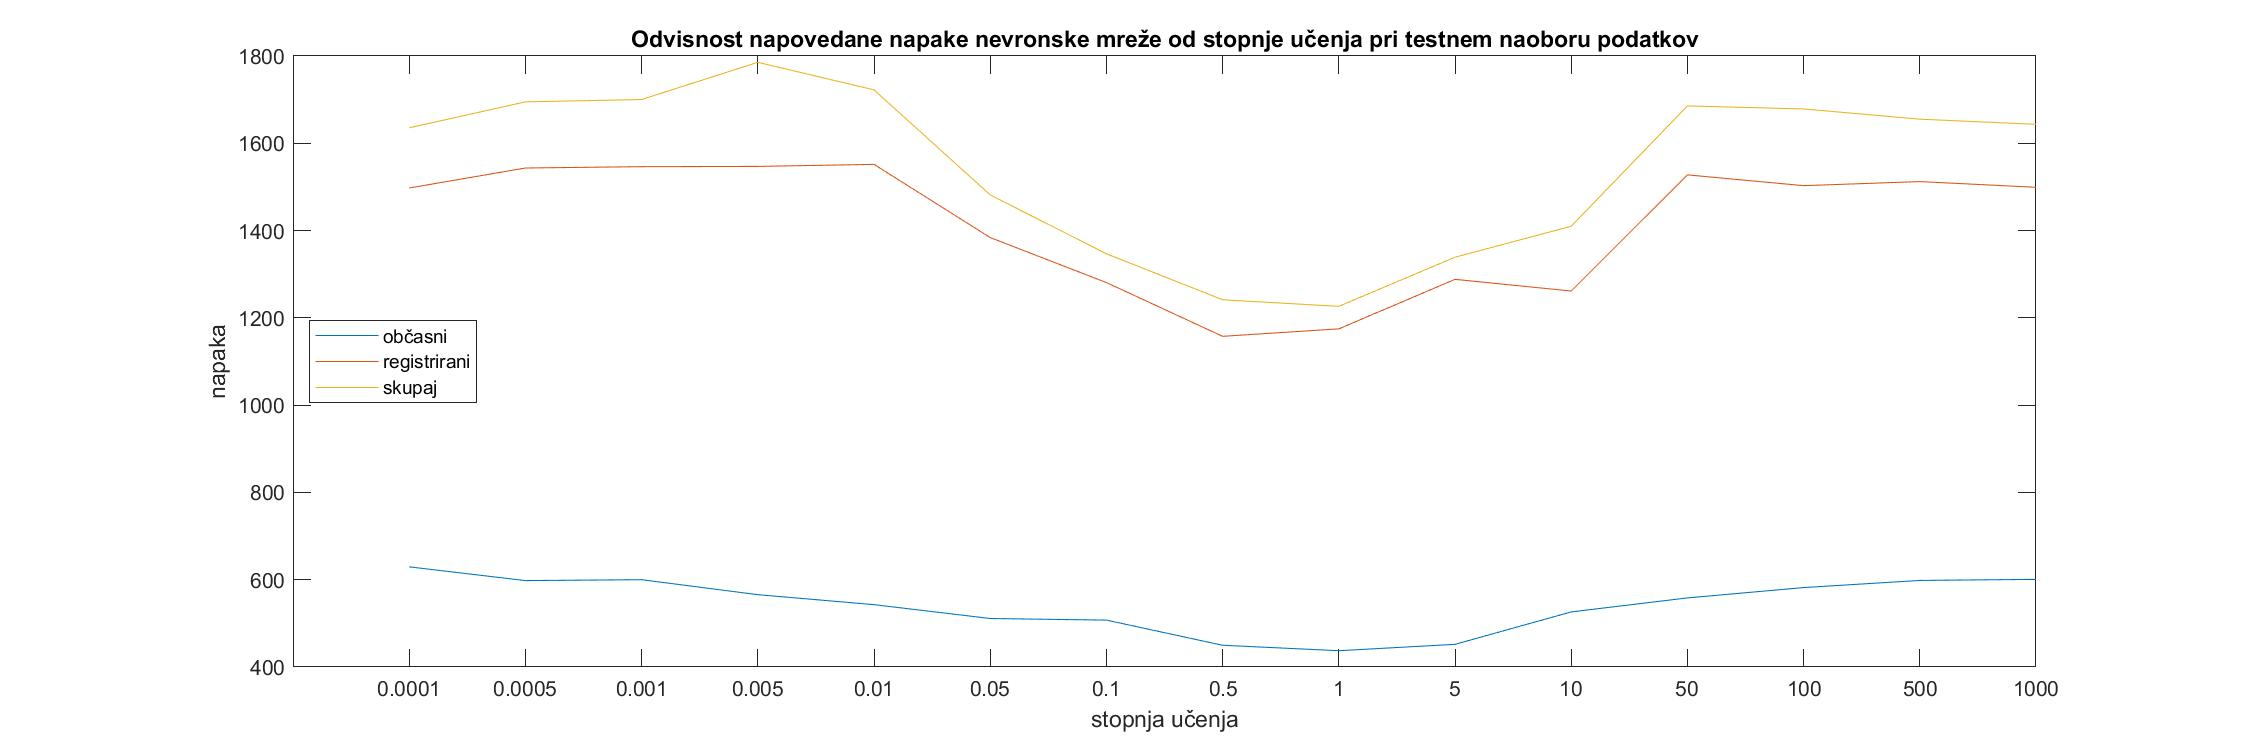
\includegraphics[width=1\textwidth]{rate.jpg}
	\caption{Vpliv stopnje učenja na učenje nevronske mreže.}
	\label{fig:rate}
\end{figure}

\subsubsection{Analiza vpliva parametrov pri učenju nevronske mreže}
Zanimalo me je, kako stopnja učenja vpliva na delovanje nevronske mreže. Pri fiksni topologiji z eno skrito plastjo z desetimi nevroni sem spreminjala stopnjo učenja. Iz grafa na sliki~\ref{fig:rate}, ki prikazuje povprečno absolutno napako pri petdesetih ponovitvah učenja v odvisnosti od stopnje učenja, je razvidno, da je napaka najmanjša, pri vrednostih $\eta = 0.5$ in $\eta = 1$. Kar je, glede na vpliv stopnje učenja pri gradientnem iskanju, povsem pričakovano.

\begin{figure}[!ht]
	\centering
	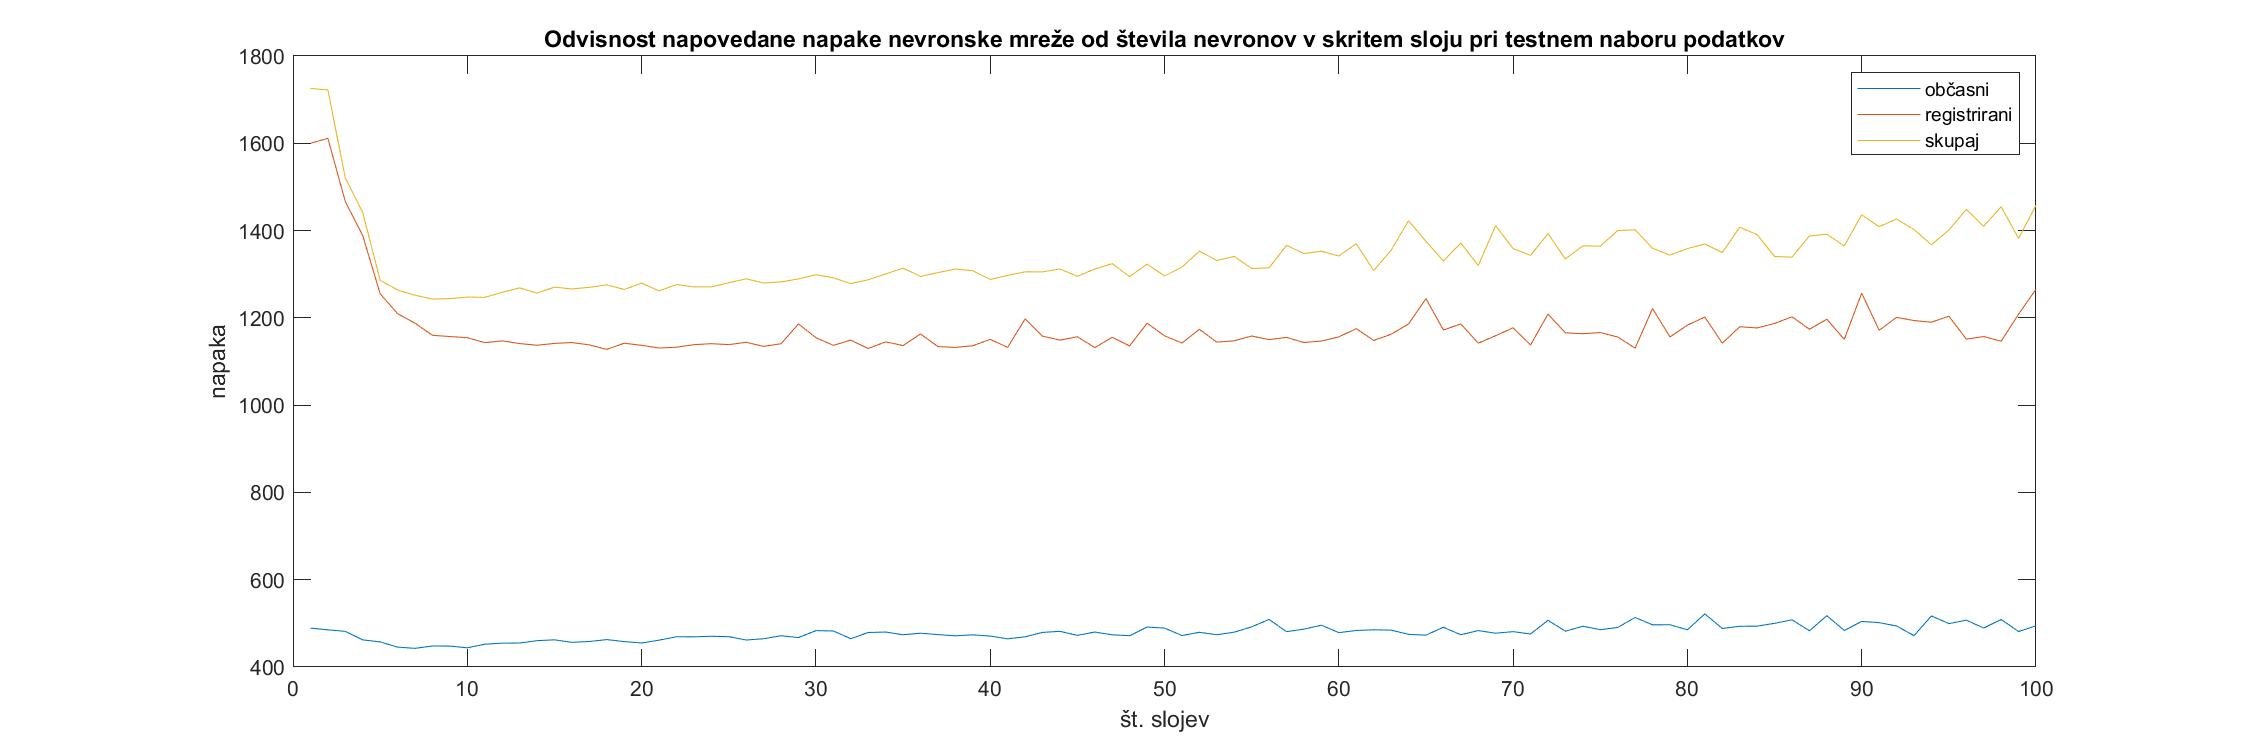
\includegraphics[width=1\textwidth]{lay.jpg}
	\caption{Vpliv števila nevronov v enem skritem sloju na učenje nevronske mreže.}
	\label{fig:lay}
\end{figure}
%test rate je pri topologiji 11,10,3
%test top je pri stopnji učenja 0.5
Nadalje sem analizirala, kakšna bi bila najbolj optimalna topologija za delovanje nevronske mreže. To sem testirala tako, da sem pri fiksni stopnji učenja $\eta = 0.5$ spreminjala število skritih nevronov. Ostala pa sem le pri enem skritem sloju, saj gre za relativno majhen podatkovni nabor in bi bila topologija z več skritimi sloji že prekompleksna, kar se kaže s slabim delovanjem nevronske mreže in posledično veliko napako pri napovedovanju. 
Graf na sliki~\ref{fig:lay} prikazuje povprečno absolutno napako pri petdesetih ponovitvah učenja v odvisnosti števila skritih nevronov. Iz grafa je razvidno, da je napaka najmanjša pri topologiji z med pet in deset nevroni v skritem sloju.

Namesto na testni podatkovni množici lahko napako izračunamo na učni podatkovni množici, tako dobimo učno napako. Graf na sliki~\ref{fig:rate_l} prikazuje vpliv stopnje učenja na učno napako, medtem ko graf na sliki~\ref{fig:lay_l} prikazuje vpliv števila skritih nevronov. Če omenjena grafa primerjamo z grafoma na slikah~\ref{fig:rate} in~\ref{fig:lay}, ugotovimo, da je pri manj kot sedmih nevronih v skritem sloju učna napaka manjhna, testna pa velika. Tako v omenjenem primeru pride do preprileganja. Podobno do preprileganja pride, v kolikor za parameter $\eta$ izberemo vrednosti večje od $50$. Do podprilegnja pride, ko je že učna napaka velika, to se zgodi pri topologijah z več kot $15$ nevroni v skritem sloju.
%
\begin{figure}[!h]
	\centering
	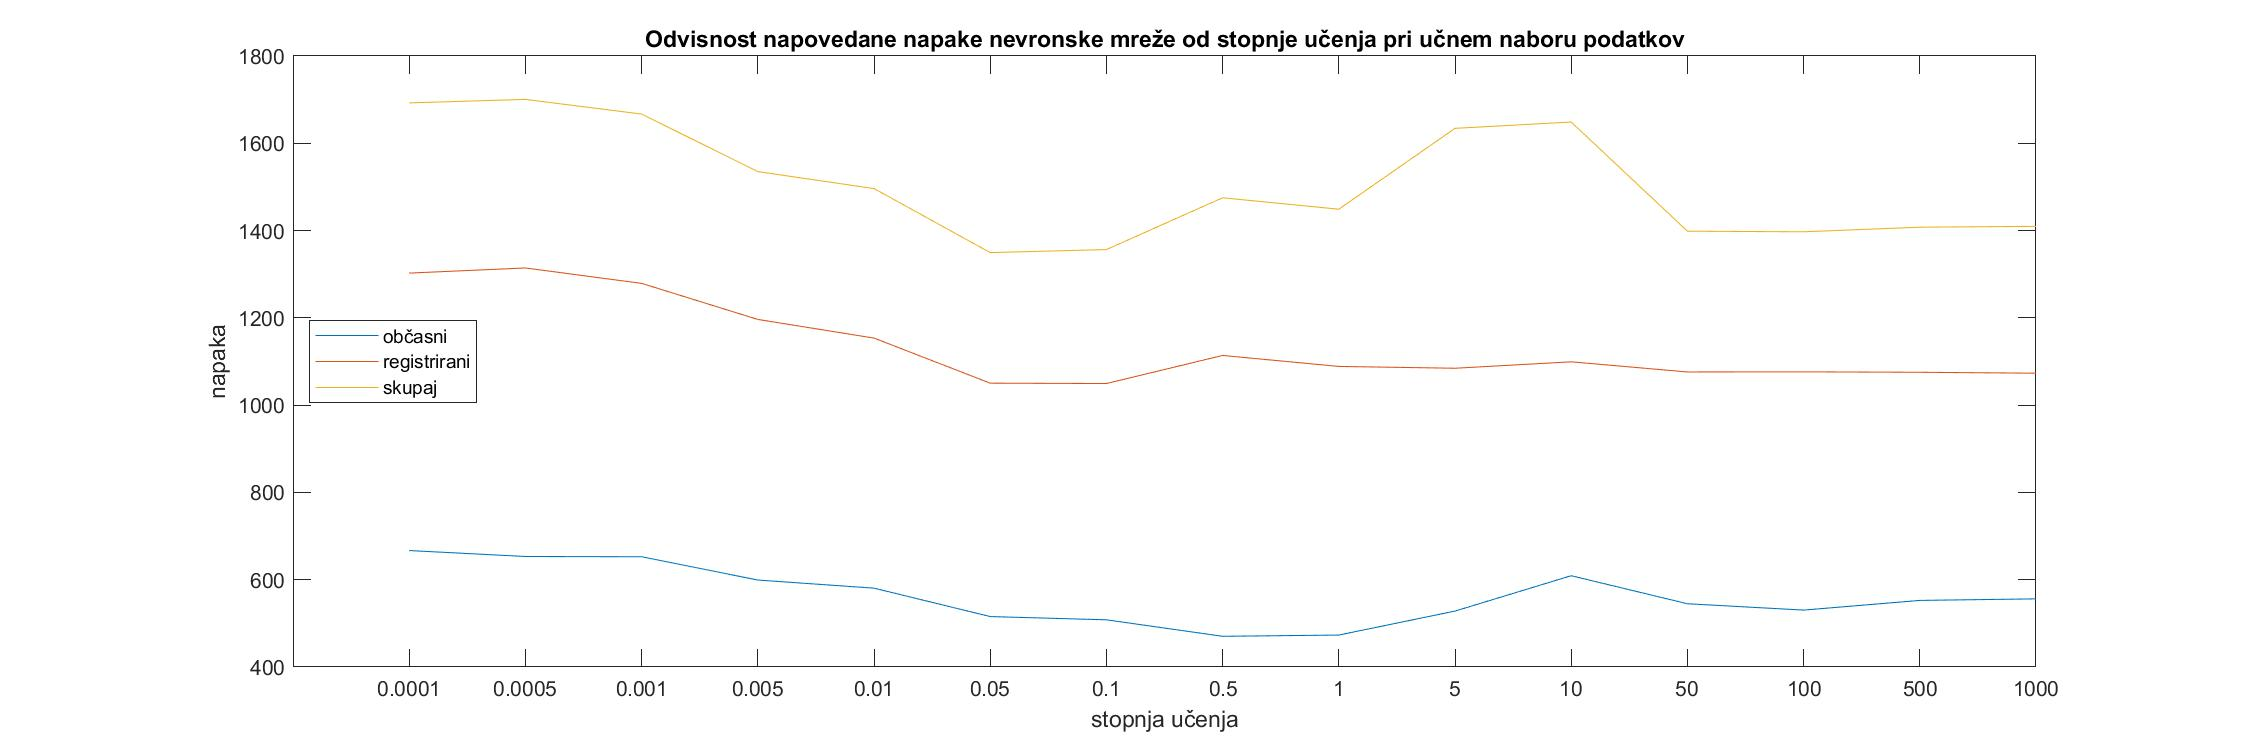
\includegraphics[width=1\textwidth]{rate_learn.jpg}
	\caption{Vpliv stopnje učenja na učenje nevronske mreže.}
	\label{fig:rate_l}
\end{figure}
%
\begin{figure}[!ht]
	\centering
	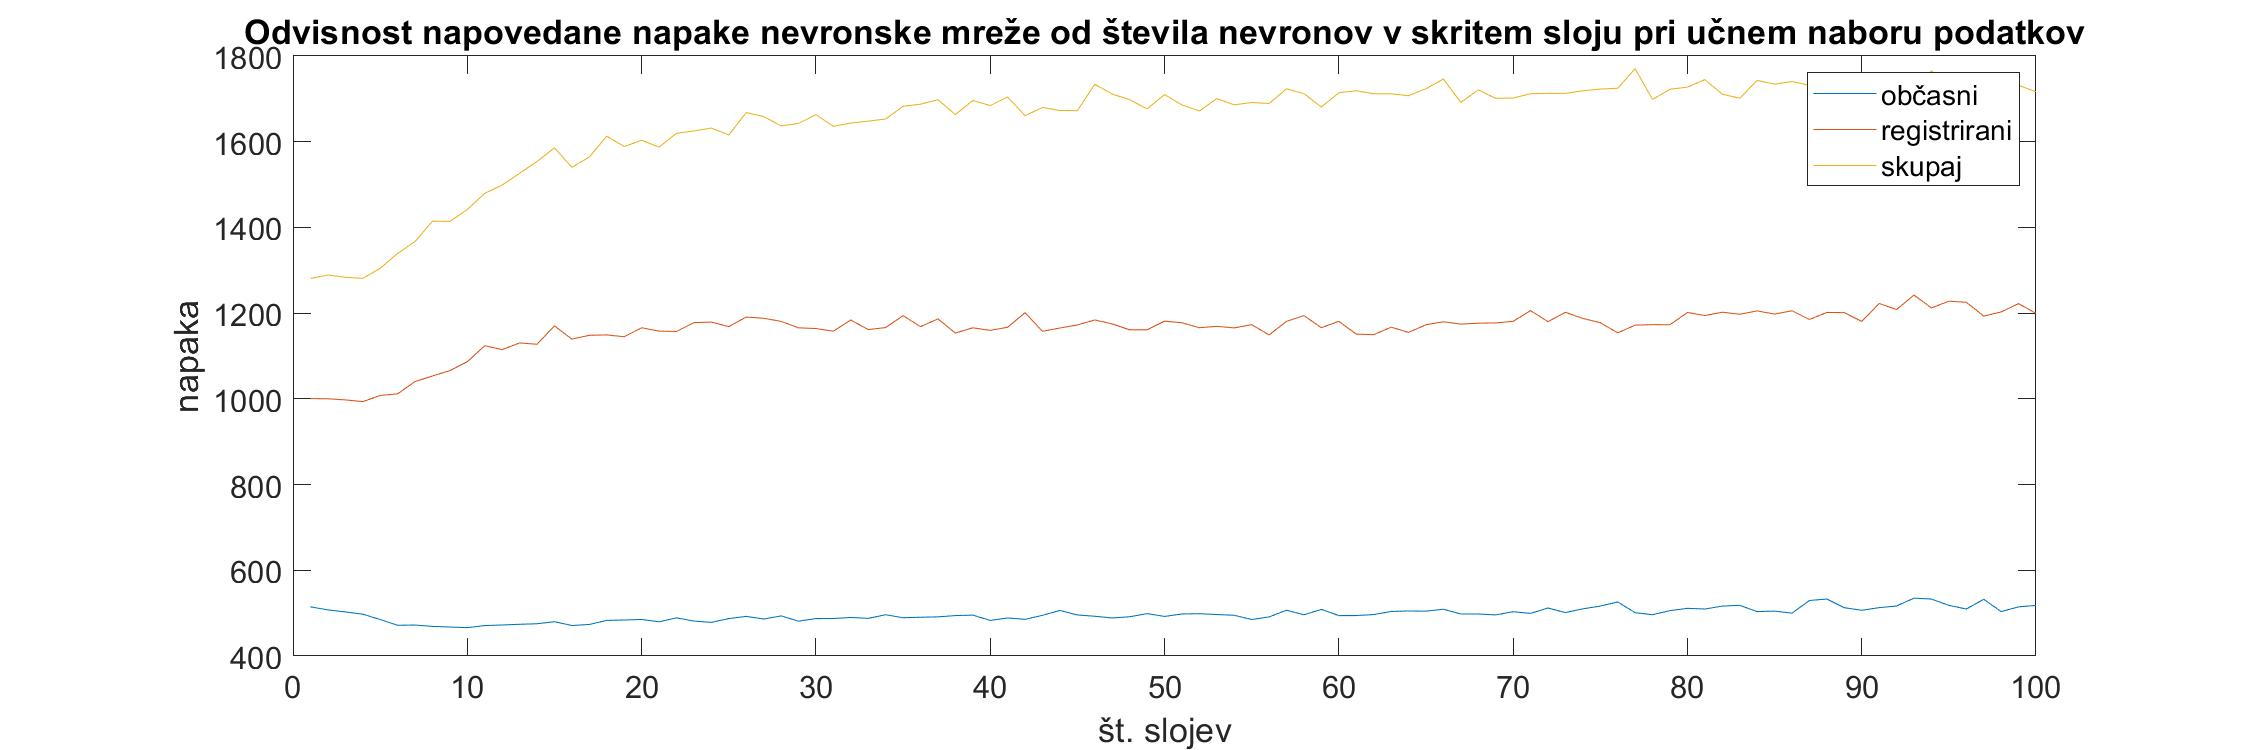
\includegraphics[width=1\textwidth]{lay_learned.jpg}
	\caption{Vpliv števila nevronov v enem skritem sloju na učenje nevronske mreže.}
	\label{fig:lay_l}
\end{figure}
%
Zaključimo lahko, da bo mreža najbolje delovala, če bo skriti sloj vseboval okoli $10$ nevronov, za stopnjo učenja pa bomo izbrali vrednost med $0.5$ in $0.1$.
%
\section{Priloga} \label{priloga}
\inputminted{ocaml}{nevronske_mreze.ml}

\section*{Slovar strokovnih izrazov}
%
\geslo{backpropagation}{vzvratno razširjanje napake}
\geslo{bias (neuron)}{(nevron) konstante aktivacije}
\geslo{bias (value)}{pristranskost (v statističnem smislu)} 
\geslo{black box model}{model, katerega delovanje težko razložimo}
\geslo{feed-forward (neural network)}{usmerjena (nevronska mreža)}
\geslo{higher-order functions}{funkcije višjega reda}
\geslo{overfitting}{preprileganje}
\geslo{pure function}{čista funkcija}
\geslo{supervised learning}{nadzorovano učenje}
\geslo{step function}{stopničasta pragovna funkcija}
\geslo{undeffitting}{neprileganje}
%\geslo{}{}


% seznam uporabljene literature
\begin{thebibliography}{99}
%
\bibitem{kononenko}I.~Kononenko in M.~ Kukar, \emph{Machine Learning and Data Mining: Introduction to Principles and Algorithms}, Horwood Publishing Limited, UK, 2007
%
\bibitem{mreze1}\emph{Neural networks}, [ogled 15.~4.~2020], dostopno na \url{https://cs.stanford.edu/people/eroberts/courses/soco/projects/neural-networks/History/history1.html}.
%
\bibitem{fact}\emph{Understanding activation functions in neural networks}, v: Medium, [ogled 20.~4.~2020], dostopno na \url{https://medium.com/the-theory-of-everything/understanding-activation-functions-in-neural-networks-9491262884e0}.
%
\bibitem{bias}\emph{Neural network bias: bias neuron, overfitting and underfitting}, [ogled 25.~4.~2020], dostopno na \url{https://missinglink.ai/guides/neural-network-concepts/neural-network-bias-bias-neuron-overfitting-underfitting/}.
%
\bibitem{intro}S.~Sathyanarayana, \emph{A gentle introduction to backpropagation}, v: Numeric Insight, Inc Whitepaper, 2014 [ogled 20.~4.~2020], dostopno na \url{https://www.researchgate.net/publication/266396438_A_Gentle_Introduction_to_Backpropagation}
%
\bibitem{kolesa}H.~Fanaee-T in J.~Gama \emph{Event labeling combining ensemble detectors and background knowledge}, v:  Progress in Artificial Intelligence (2013): pp. 1-15, Springer Berlin Heidelberg, [ogled 15.~3.~2020], dostopno na \url{https://archive.ics.uci.edu/ml/datasets/bike+sharing+dataset}.
%
\bibitem{Ocaml1} \emph{https://ocaml.org/learn/description.html}, [ogled 5.~5.~2020], dostopno na \url{https://ocaml.org/learn/description.html}.
%\bibitem{Ocaml2} 
%
\bibitem{hebb}D.~O.~Hebb, \emph{The organization of behavior: A neuropsychological theory}, Wiley, New York, 1949.
%
\bibitem{rosenblatt}F.~Rosenblatt, \emph{Principles of neurodynamics: Perceptrons and the theory of brain mechanisms}, Spartan Books,  Washingotn, D.C., 1962.
%
\bibitem{grad}\emph{Learning rate gradient descent}, [ogled 12.~6.~2020], dostopno na \url{https://saugatbhattarai.com.np/what-is-gradient-descent-in-machine-learning/learning-rate-gradient-descent/}.
\end{thebibliography}

\end{document}

